\documentclass{beamer}
\setbeamertemplate{navigation symbols}{}

\usepackage{beamerthemeshadow}
\usepackage{amsmath}
\begin{document}
\title{Training a dynamical system by using multivariate information}  
\author{Clayton Seitz}
\date{\today} 

\begin{frame}[plain]
\titlepage
\end{frame}

\begin{frame}[plain]\frametitle{Table of contents}\tableofcontents
\end{frame} 

\section{Introduction} 

\begin{frame}[plain]
\frametitle{Introduction} 

Neuroethology argues that neural networks evolve according to the stimuli to which they are exposed

\begin{center}
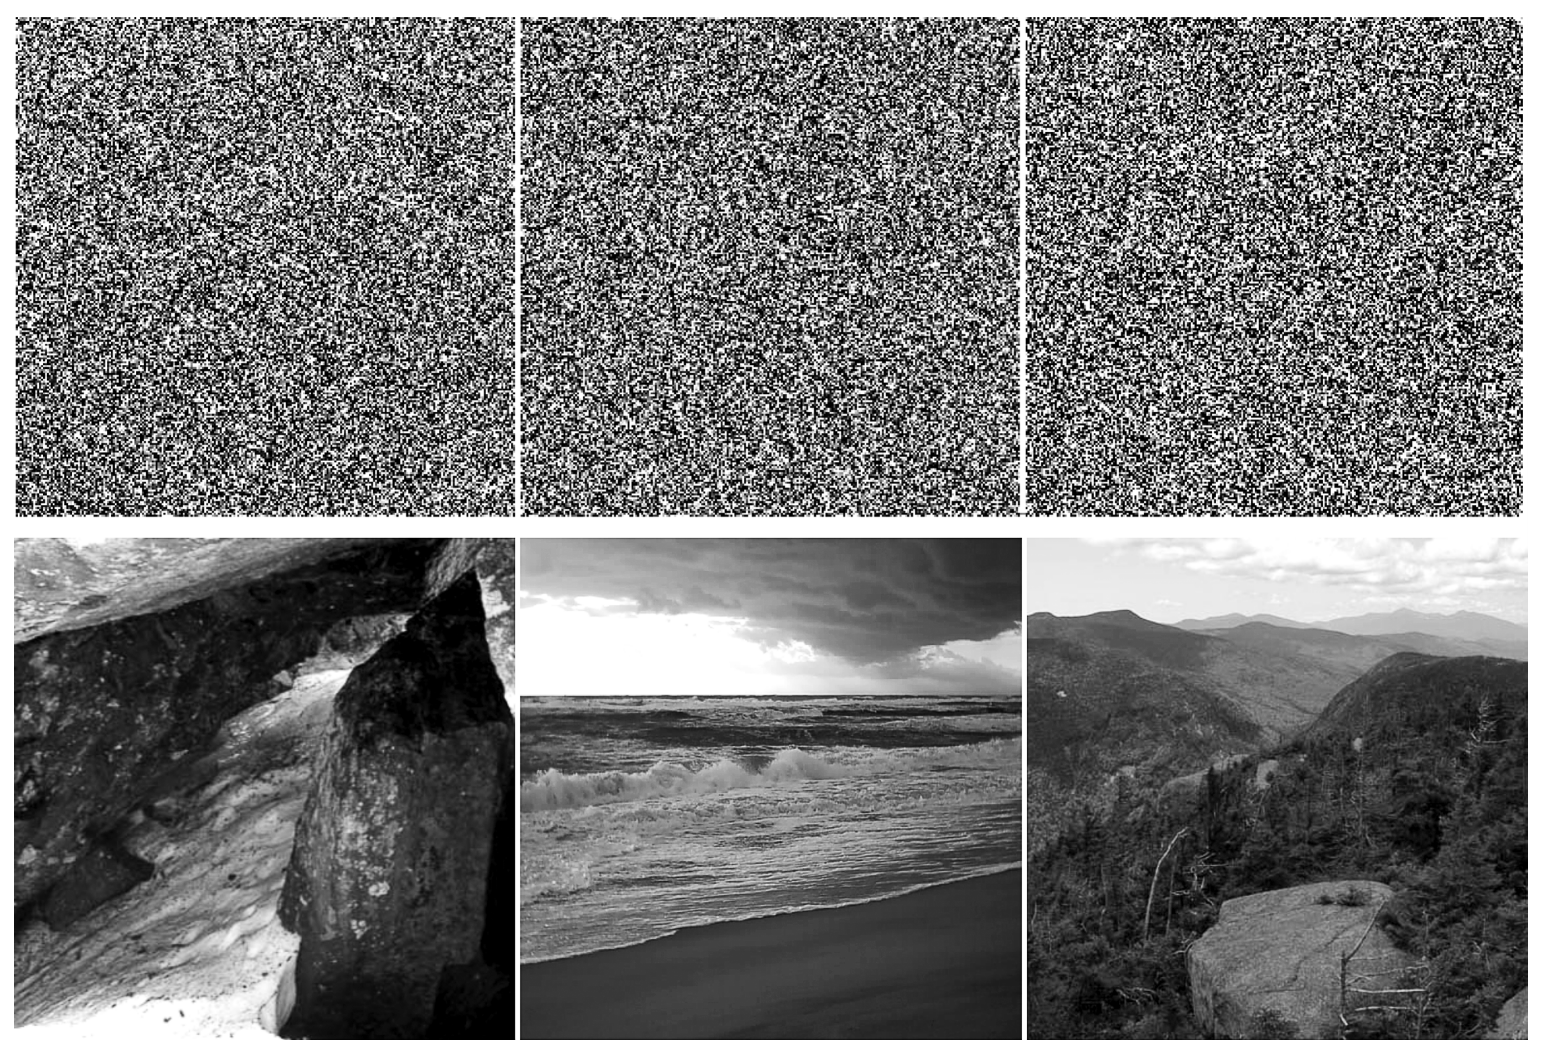
\includegraphics[scale=0.35]{natural-images}
\end{center}

\end{frame}


\section{Channel coding for neural networks} 

\begin{frame}[plain]
\frametitle{Channel coding for neural networks} 

Networks of neurons can be viewed as a communication channel

Except this communication channel \emph{learns} the transformation $F$ based on the statistical structure of its input $X$. Visual cortex has learned an encoding for visual scenes (that perhaps maximizes information)

\end{frame}


\section{Supervised training of low-rate critical networks} 

\begin{frame}[plain]
\frametitle{Leaky integrate and fire neurons} 

A realistic LIF model might look like

\begin{equation*}
\tau_{m}\frac{d\mathbf{V}[I]}{dt} = (\mathbf{V}[I]-E)\sum_{j} \mathbf{W^{0}}[I,j] + (\mathbf{V}[I] - E_{in})\sum_{k}\mathbf{W^{1}}[I,k])
\end{equation*}

Instead, we ignore changes in the voltage of the postsynaptic neuron due to subthreshold voltages of the presynaptic neuron and let matrices $\mathbf{W}$ learn the input-output voltage relationship

\begin{equation*}
V[j,t+1] = \alpha V[j,t+1] + \sum_{i\neq j} W^{0}_{ij}z[i,t] + \sum_{i} W^{1}_{ij}x[i,t+1] - z[j,t]v_{th} 
\end{equation*}

where $z = H(v-v_{th})$


\end{frame}


\begin{frame}[plain]
\frametitle{Estimating gradients} 

Say we have a model $\Phi = (W^{0},W^{1})$ and want to use gradient descent to train a network to have a target rate or a target branching parameter. The rate and its associated loss for a single unit is

\begin{equation*}
r(t) = \frac{1}{\Delta t}\int_{t}^{t+\Delta t} d\tau \langle \rho(\tau)\rangle\;\;\;\;\;\mathcal{L} = \alpha(r-r_{0})^{2}
\end{equation*}

We would like the standard update 

\begin{equation*}
\Delta W_{ij} = -\eta \frac{\partial\mathcal{L}}{\partial W_{ij}}
\end{equation*}


But it is intractable to compute $\frac{\partial\mathcal{L}}{\partial W_{ij}}$ since $\rho(t)$ depends on other neurons through space and time.


\end{frame}


\begin{frame}[plain]
\frametitle{Estimating gradients} 

Bellec et al. presented a solution to estimating $\frac{\partial\mathcal{L}}{\partial W_{ij}}$ for online learning, but it can just as well be used for supervised learning

\begin{equation*}
\frac{\partial\mathcal{L}}{\partial W_{ij}} = \sum_{t} \frac{\partial \mathcal{L}}{\partial z[j,t]} \cdot \frac{\partial z[j,t]}{\partial W_{ij}}
\end{equation*}

where the gradient $\frac{\partial z[j,t]}{\partial W_{ij}}$ is computed locally.




\end{frame}

\section{Multivariate information theory} 

\begin{frame}[plain]
\frametitle{Multivariate information theory} 
\end{frame}

\section{Adaptation of the transfer function} 

\begin{frame}[plain]
\frametitle{Adaptation of the transfer function} 
How do neuron transfer functions adapt to stimuli in an unsupervised manner?
\end{frame}

\section{Learning an energy function over phase space} 

\begin{frame}[plain]
\frametitle{Adaptation defines an energy function over phase space} 
\end{frame}

\section{Generalization bounds and density estimation} 

\begin{frame}[plain]
\frametitle{Generalization bounds}
What is the distance of a code defined by a particular energy function $\mathbf{E}$
\end{frame}

\section{The energy function defines a dynamical system} 

\begin{frame}[plain]
\frametitle{The energy function defines a dynamical system} 
\end{frame}


\section{The energy function is a generative model} 

\begin{frame}[plain]
\frametitle{The energy function is a generative model} 
\end{frame}

\section{Application to natural image statistics} 

\begin{frame}[plain]
\frametitle{Application to natural image statistics} 
\end{frame}





\end{document}